
\subsection{Батиметрия}

Опираясь на рассмотренные в разделах~\ref{sec:seashoaring} и~\ref{sec:wave_refraction} формулы ясно, что для корректного расчета показателей волновой энергии необходимым условием является наличие профиля морского дна вдоль рассматриваемого направления.
Получение необходимых профилей может быть выполнено при условии наличия результатов батиметрических съемок -- «топографических» карт морского дна.
Аналогично топографическим изысканиям, батиметрия дна может выполняться с применением различных методов, начиная от примитивных классических лот-съемок и заканчивая привлечением технологий спутниковошо и лахерно-сканирующего зондирования.

Несмотря на то, что качественная батиметрия является фундаментом для морской навигации, океанографии, геодинамики и климатологии на сегодняшний день сложилась парадоксальная ситуация, когда поверхность Луны и Марса картирована значительно подробнее и детальнее дна земных морей и океанов.
Ответы о причинах и следствиях указанного факта отчасти лежат в историческом контексте поиска и накопления этих данных.
История формирования батиметрических данных -- это история компромисса между физическими ограничениями измерительных технологий, масштабами Мирового океана и международной политической волей к обмену результатами съемок.
Не смотря на кажущуюся избыточность изложения не откажем себе в любопытстве и удовольствии погрузиться в рассмотрение этого материала подробнее!

\subsubsection{История мировой батиметрии}

Интерес к получению батиметрических данным не ослабевает на протяжении с последних двух веков.
Систематическое картирование глубин Мирового океана началось во второй половине XIX века. 
Необходимость глобального картирования морского дна встала перед человечеством в моменты возникновения первых глобальных задач.
Так прокладка трансатлантического телеграфного кабеля в 1858-1866 годах сформировала инженерную необходимость систематической съемки дна Северной Атлантики, став одним из условий установления постоянной связи между материками.

Международная институционализация батиметрических данных связана с именем Альбера I, князя Монако. 
В 1903 году по его инициативе была учреждена организация General Bathymetric Chart of the Oceans (GEBCO).
Основу первого издания GEBCO составили сводные батиметрические материалы, предоставленные национальными гидрографическими службами ведущих морских держав того времени (прежде всего Великобритании, Франции, Германии, России, США и Японии).
Выпускавшиеся вплоть до 1980-х годов бумажные карты GEBCO заложили традицию международного обмена батиметрическими данными. 
И сегодня архив этих исторических бумажных карт доступен через сайт Международной Гидрографической Организации (МГО), хотя, по очевидным причинам, не является удобным для автоматической обработки и использования в данной работе.

Первые попытки обобщения батиметрических съемок выполнялись вручную по данным разрозненных и одиночных измерений, полученных методом лотового промера.
Естественная простота этого способа измерений определяла его доступность для человечества многие века.
Однако свойственная ему редкая сеть измерений делает этот способ эффективным лишь для локально ограниченных участков прибрежных территорий (промеров портов, озер, гидроотвалов и~т.\,п.).

Изобретение акустического эхолота в 1920-х годах кардинально изменило возможности батиметрической съемки. 
Если лотовый промер позволял получать данные со скоростью несколько точек в час, то эхолот начал формировать непрерывный профиль глубин вдоль курса судна. 
Многолучевые эхолоты (MultiBeam Echo Sounder (MBES)), получившие широкое распространение в научных экспедициях начиная с 1970–1980-х годов, принципиально изменили подход к съемке. 
В отличие от однолучевых систем, MBES одновременно излучает и принимает множество акустических лучей, формируя поперечную полосу относительно трассы съемки. 
На сегодняшний день точность MBES достигает 0,2–0,3\% от глубины, что обеспечивает погрешность измерений порядка нескольких метров даже на глубинах 4–5 км.
Сегодня именно многолучевая съемка постепенно становится технологическим стандартом как для научных экспедиций так и производственных работ.
Однако несмотря на совершенствование как приборной, так и методической базы высокая стоимость и трудоемкость работ объясняют печальный факт того, что сегодня методами прямых батиметрических измерений покрыто лишь около 28,7\% площади дна Мирового океана.

Принципиально важным прорывом в батиметрии стала разработка методов предсказания глубин по данным спутниковой радарной альтиметрии. 
Физическая идея метода состоит в том, что рельеф морского дна создает локальные аномалии поля силы тяжести, деформируя геоид (среднюю уровневую поверхность океана) на величины порядка первых сантиметров.
Высокоточный альтиметр способен зафиксировать эти отклонения, позволяя косвенно пересчитать их в оценки топографии дна.
Пионерами этого метода стали В. Смит и Д. Сандвелл (Scripps Institution of Oceanography). 
В своей работе~\cite{SmithSandwell1994} они показали принципиальную возможность восстановления глобальной батиметрии морского дна по альтиметрическим данным, а в 1997 году опубликовали первую глобальную предиктивную модель~\cite{SmithSandwell1997}.

На протяжении XX века все главные океанографические службы мира (National Oceanic and Atmospheric Administration (NOAA), Scripps Institution of Oceanography, Woods Hole Oceanographic Institution, а также советские научно-исследовательские и экспедиционные суда «Персей», «Витязь», «Академик Курчатов» и~др.) накапливали данные, постепенно заполняя ими поверхность Мирового океана.

Центральным хранилищем этого наследия стал IHO Data Centre for Digital Bathymetry (DCDB), основанный в 1990 году и размещенный в NOAA в Боулдере, Колорадо. 
Сегодня архив DCDB содержит свыше 70 терабайт данных одно- и многолучевых зондирований. Данные из этого архива предоставляются свободно и без ограничений.

В 1980-х годах NOAA (тогда Национальный геофизический центр данных NGDC) приступил к разработке серии глобальных батиметрических и топографических растров, объединенных под именем ETOPO (Earth TOPOgraphy). 
Первый продукт серии -- ETOPO5 с разрешением 5 угловых минут (≈9,3 км на экваторе) был компиляцией разрозненных национальных данных и имел существенные погрешности, особенно в районах со слабой изученностью.
В 1990-е годы появился ETOPO2, выполненный с угловым разрешением в 2 угловые минуты, а в 2009 году ETOPO1 с разрешением 1 угловая минута (≈1,8 км). 
ETOPO1 объединял топографию SRTM30 над сушей с данными многолучевой эхолокации и спутниковой альтиметрии.

Последняя версия серии ETOPO 2022 сформирована с разрешением 15 угловых секунд (≈500 м на экваторе), используя в качестве базы батиметрию ICESat-2, данные воздушных лидарных съемок, спутникового зондирования и корабельных промеров. 
Продукт выпускается в версиях  Ice Surface и Bedrock, предоставляясь бесплатно через NOAA NCEI.

Параллельно с ETOPO развивалась цифровая ветвь GEBCO. 
Передав сопровождение продуктов организации Британскому океанографическому центру данных (BODC) в 1990 году, GEBCO в 2003 году выпустила свою первую глобальную батиметрическую модель GEBCO One Minute Grid с разрешением в 1 угловую минуту. 
В 2009 году появилась модель GEBCO\_08 Grid с разрешением 30 угловых секунд, основанная на комбинации прямых корабельных промеров и косвенных глубин, полученных по спутниковым данным.

С 2019 года, в рамках проекта Nippon Foundation-GEBCO Seabed 2030, GEBCO ежегодно публикует уточненные данные с разрешением 15 угловых секунд. 
Последовательно выходили GEBCO\_2019-2025 и в апреле 2026 года -- GEBCO\_2026. 
Данные публикуются в форматах NetCDF, GeoTIFF и Esri ASCII Raster и распространяются свободно в качестве публичного достояния.

Не вдаваясь в подробности, следует отметить, что параллельно с глобальными моделями развиваются и региональные проекты, ориентированные на конкретные акватории с особым научным или практическим статусом.

Инициатива International Bathymetric Chart of the Arctic Ocean (IBCAO) основана в 1997 году и с тех пор является наиболее авторитетным источником батиметрии для районов севернее 64° с.ш.
Исходные данные охватывают период с 1950-х до 2020-х годов и включают многолучевые и однолучевые эхолоты, оцифрованные контуры архивных карт и данные ледокольных экспедиций. 
International Bathymetric Chart of the Southern Ocean (IBCSO) -- аналогичная инициатива для районов южнее 50° ю.ш., координируемая Институтом Альфреда Вегенера (AWI).

European Marine Observation and Data Network Bathymetry (EMODnet) -- инициатива Европейской комиссии, предоставляющая согласованные цифровые модели рельефа (DTM) европейских морских бассейнов. 
Выпуск DTM 2024 основан на 22 032 съемочных наборах данных, поступивших от 66 организаций из 28 стран. 
Разрешение продукта составляет 1/16 угловой минуты (≈115 м), а в районах с плотной съемкой доступны составные DTM с разрешением до 1/512 угловой минуты.
Важно отметить, что в зону EMODnet (рисунок~\ref{pic:emodnet}) попадают акватории Черного, Балтийского, Белого и Баренцева морей~\cite{emodnet_geoviewer}, что делает эту модель потенциально применимой для анализа прибрежных территорий России.

\begin{figure}
    \begin{center}
	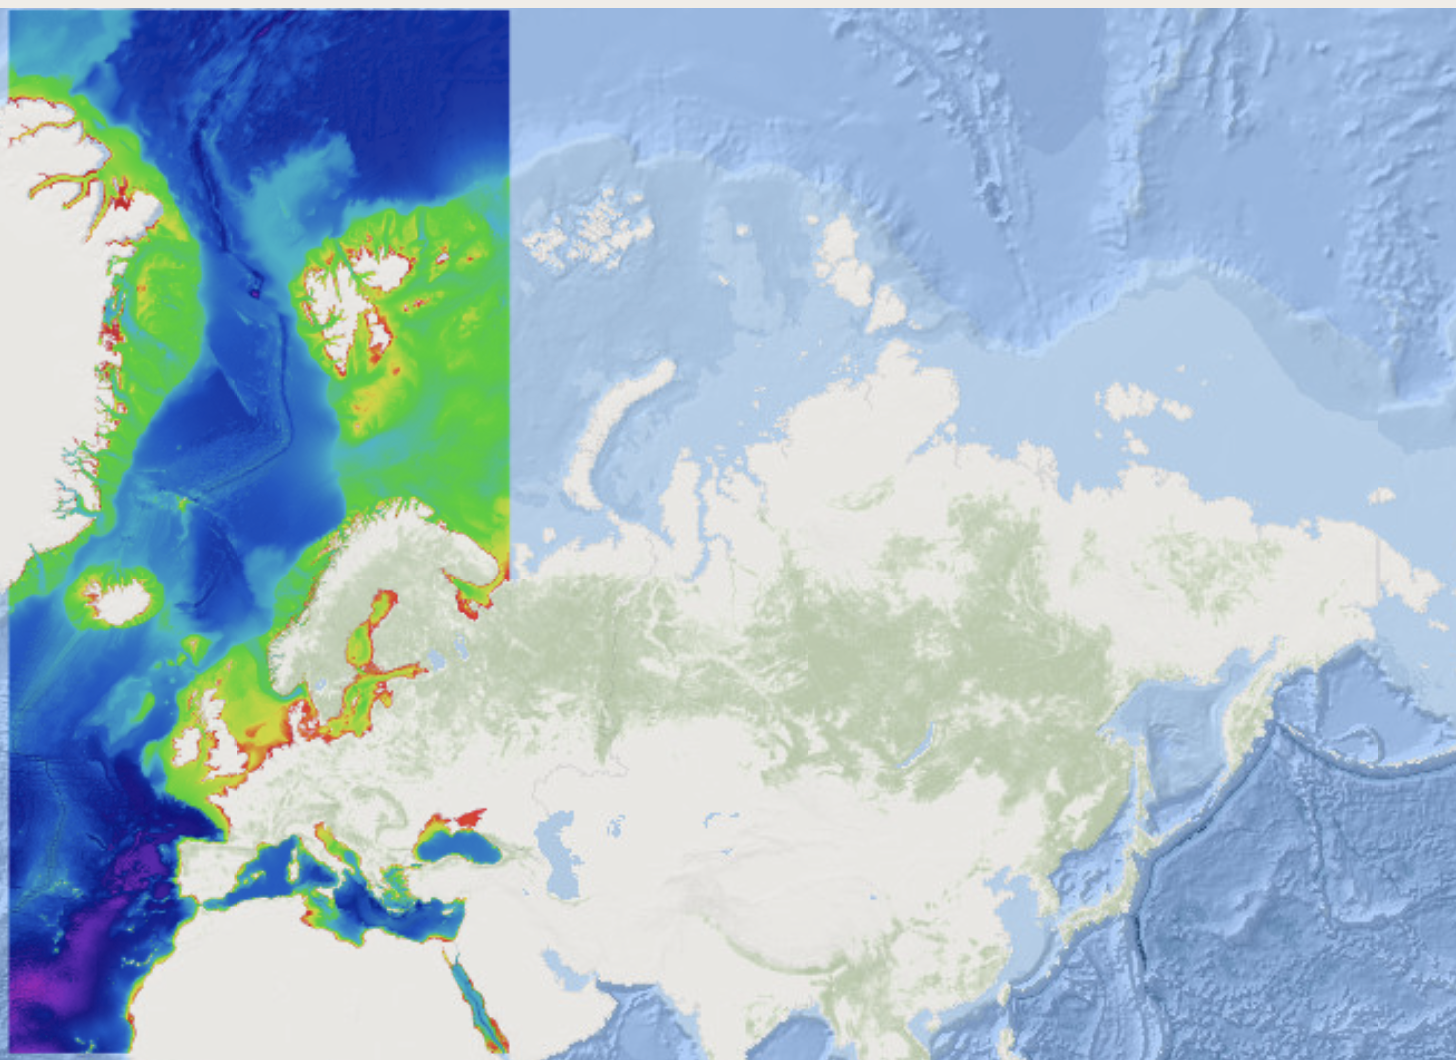
\includegraphics[width=100mm]{fig/part_2/EMODnet.png}
	\caption{-- Область батиметрических данных EMODnet относительно территории РФ~\cite{emodnet_geoviewer}}
	\label{pic:emodnet}
    \end{center}
\end{figure}

\subsubsection{Инструменты доступа и получения данных}
\label{sec:bathy_source}

Рассматривая автоматизированные способы получения батиметрических данных можно условно классифицировать их на три уровня:
\begin{itemize}
    \item готовые высокоуровневые библиотеки;
    \item веб-сервисы на основе REST (Representational State Transfer) и стандартов OGC (Open Geospatial Consortium);
    \item прямой доступ к растровым файлам.
\end{itemize}

Библиотеки верхнего уровня являются по сути обертками API глобальных моделей рельефа. 
Типичный пример -- PyGMT, которая фактически служит фронтом к серверу данных GMT с моделями GEBCO и SRTM15+. 
Указав требуемые границы, угловое разрешение и источник библиотека формирует необходимые запросы и загружает нужный фрагмент, кэшируя его и возвращая в виде xarray-объекта. 

Прямой вызов веб-сервисов, отдающих батиметрию по HTTP является наиболее гибким каналом для получения данных из сервисов, распространяющие модели через REST API, не входящие в перечень доступных через PyGMT. 
Принципиально такая модель запроса напрямую позволяют запросить произвольный прямоугольник по координатам и получить ответ в формате GeoTIFF, либо NetCDF. 

Центр CEDA (Великобритания) предоставляет доступ к глобальным моделям GEBCO по протоколу OPeNDAP, позволяющему прямо обращаться к выборкам данных из приложений -- без скачивания полного файла. 
EMODnet поддерживает OGC-сервисы WMS, WCS, WFS и WMTS для европейских акваторий. 
PANGAEA предоставляет доступ к архиву многолучевых данных через собственный WMS/WFS.
Обработка данных на стороне клиента выполнятеся средствами пакетов \texttt{xarray} (для NetCDF/OPeNDAP) и rasterio/GDAL (для растров). 

В рамках выполняемой работы важно, что все перечисленные источники покрывают основной набор акваторий страны через глобальные модели, такие как GEBCO и ETOPO.
Эти модели предоставляют данные для всего Северного Ледовитого океана, Дальневосточных морей и внутренних морей.
В тоже время европейские и региональные продукты дополняют их данными с повышенным разрешением. 
При этом python-стек (\texttt{xarray}, \texttt{rasterio}, \texttt{PyGMT}, \texttt{GeoPandas} и различные REST-клиенты) позволяет строить полностью автоматизированные конвейеры, начинающиеся с загрузки нужного фрагмента модели и продолжающиеся операциями перепроецирования, фильтрации и подготовки данных для последующих вычислений.

\subsubsection{Заключение}

На протяжении более чем ста лет -- от бумажных карт принца Альбера I до ежегодных цифровых обновлений GEBCO\_2026 открытые батиметрические данные прошли путь от разрозненных национальных коллекций к единой международной инфраструктуре. 
Ключевыми вехами этого пути стали основание GEBCO в 1903 году, технологический переход от лота к эхолоту и многолучевым системам, пионерские работы Смита–Сандвелла по гравиметрической инверсии в 1990-х годах, запуск проекта Seabed 2030 в 2017-м, появление ICESat-2 ATL24 в 2025-м и начало эры SWOT-батиметрии. 
Вместе с тем выполненный анализ показывает, что значительная часть «глобальных» моделей остается предиктивной интерполяцией, а не прямым измерением, что диктует необходимость осознанного выбора источника данных в зависимости от конкретного типа решаемой задачи.
